\documentclass[12pt]{article}

\usepackage[utf8]{inputenc}
\usepackage[margin=1in]{geometry}
\usepackage{graphicx}
\usepackage{booktabs} 
\usepackage{float}    
\usepackage{caption}

\title{Assignment 4 - Part 2: Object Detection Model Comparison}
\author{Jana Adel 8273 Shahd Sherif 8145}
\date{24th of June 2025}

\begin{document}

\maketitle

\section*{Model Comparison and Analysis}

This section presents an in-depth comparison of three prominent object detection models: \textbf{Faster R-CNN}, \textbf{SSD}, and \textbf{YOLOv5}. The comparison considers both the underlying architecture and practical inference results on COCO validation images. Each model was run on a fixed subset of images, and results were evaluated visually and analytically.

\subsection*{1. Faster R-CNN}
Faster R-CNN is a two-stage object detection model proposed by Ren and others in 2015. It significantly improved detection accuracy compared to earlier methods.

\begin{itemize}
    \item \textbf{Backbone:} ResNet-50 with Feature Pyramid Network (FPN).
    \item \textbf{Stage 1:} A Region Proposal Network (RPN) scans the image to propose candidate object regions.
    \item \textbf{Stage 2:} These regions are fed into a classification and bounding box regression head.
    \item \textbf{Strengths:} 
    \begin{itemize}
        \item Excellent detection performance on small and overlapping objects.
        \item High accuracy, especially in cluttered or complex scenes.
    \end{itemize}
    \item \textbf{Weaknesses:}
    \begin{itemize}
        \item Slow inference time due to its two-stage nature.
        \item Requires significant computational resources.
    \end{itemize}
    \item \textbf{Best For:} Applications where accuracy is more important than speed, e.g., medical imaging, satellite imagery.
\end{itemize}

\subsection*{2. SSD (Single Shot MultiBox Detector)}

SSD is a one-stage object detection network introduced by Liu and others in 2016. Unlike Faster R-CNN, SSD performs detection in a single pass.

\begin{itemize}
    \item \textbf{Backbone:} VGG-16.
    \item \textbf{Core Idea:} SSD predicts bounding boxes and class probabilities directly from multiple feature maps of different resolutions.
    \item \textbf{Strengths:}
    \begin{itemize}
        \item Simpler and faster than two-stage models.
        \item Performs well on medium-to-large objects.
    \end{itemize}
    \item \textbf{Weaknesses:}
    \begin{itemize}
        \item Less accurate with small and densely packed objects.
        \item The fixed set of default boxes limits localization precision.
    \end{itemize}
    \item \textbf{Best For:} Real-time applications with moderate accuracy needs, such as embedded systems.
\end{itemize}

\subsection*{3. YOLOv5}

YOLOv5 is the latest iteration of the YOLO (You Only Look Once) series, developed by Ultralytics. It provides an optimal balance between speed and accuracy using modern backbone and training strategies.

\begin{itemize}
    \item \textbf{Backbone:} CSPDarknet.
    \item \textbf{Architecture:}
    \begin{itemize}
        \item Uses a single CNN to predict bounding boxes and class probabilities across the entire image.
        \item Incorporates modern techniques like spatial pyramid pooling, path aggregation, and anchor-free prediction.
    \end{itemize}
    \item \textbf{Strengths:}
    \begin{itemize}
        \item Real-time inference speed with competitive accuracy.
        \item High performance in detecting objects at multiple scales.
    \end{itemize}
    \item \textbf{Weaknesses:}
    \begin{itemize}
        \item Occasionally over-predicts (false positives).
        \item Slightly lower accuracy than Faster R-CNN on very small objects.
    \end{itemize}
    \item \textbf{Best For:} Real-time object detection in videos, surveillance, robotics.
\end{itemize}


\subsection*{Quantitative Results}

\begin{table}[H]
\centering
\caption{Performance Comparison Summary}
\begin{tabular}{@{}l p{4cm} p{5cm} p{5cm}@{}}
\toprule
\textbf{Model} & \textbf{Speed (s/image)} & \textbf{Strengths} & \textbf{Weaknesses} \\
\midrule
Faster R-CNN & 0.5 -- 1.0 & High accuracy, small object detection & Very slow inference, needs GPU \\
SSD & 0.2 -- 0.4 & Fast and lightweight & Poor with small or overlapping objects \\
YOLOv5 & 0.04 -- 0.1 & Fast and accurate balance & False positives in background \\
\bottomrule
\end{tabular}
\end{table}


\subsection*{Qualitative Observations}

\begin{itemize}
    \item \textbf{Faster R-CNN} correctly detected overlapping persons in crowded scenes, and small distant objects (e.g., bottles, animals) were localized precisely.
    \item \textbf{SSD} performed well in detecting large cars and bikes, but often missed small objects like birds or remote people.
    \item \textbf{YOLOv5} showed balanced behavior: it was fast and detected most major objects correctly, though it occasionally produced boxes in background areas.
\end{itemize}

\subsection*{Conclusion}

Each model has specific strengths and is suited to different deployment scenarios:

\begin{itemize}
    \item Use \textbf{Faster R-CNN} when detection quality is the priority and computational cost is not a concern.
    \item Choose \textbf{SSD} for fast inference in constrained environments but avoid it for complex scenes.
    \item \textbf{YOLOv5} is a great middle-ground with state-of-the-art speed and solid accuracy for real-time use.
\end{itemize}
\section*{Results and Discussion}

\subsection*{YOLOv5 Results}

\begin{figure}[H]
    \centering
    \begin{minipage}[b]{0.45\textwidth}
        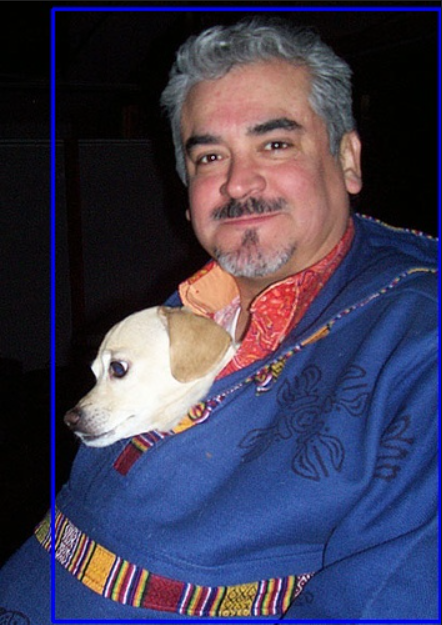
\includegraphics[width=\textwidth]{yolo_result1.png}
        \caption*{\textbf{Image 1:} YOLOv5 correctly detected the person but missed the dog due to overlap .}
    \end{minipage}
    \hfill
    \begin{minipage}[b]{0.45\textwidth}
        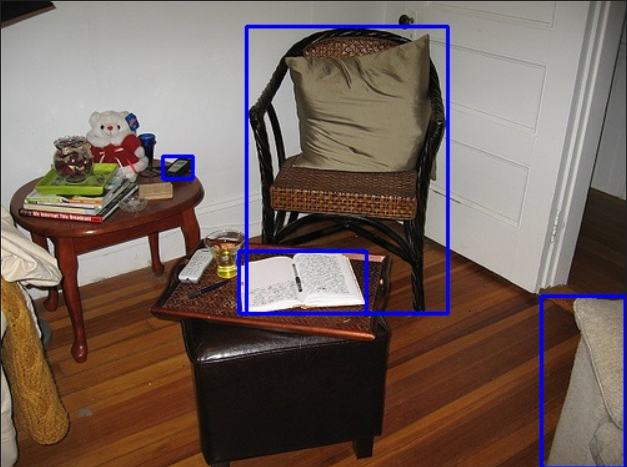
\includegraphics[width=\textwidth]{yolo_result2.png}
        \caption*{\textbf{Image 2:} missed alot of objects in the background.}
    \end{minipage}
    \caption{Sample predictions using YOLOv5}
\end{figure}

\subsection*{SSD Results}

\begin{figure}[H]
    \centering
    \begin{minipage}[b]{0.45\textwidth}
        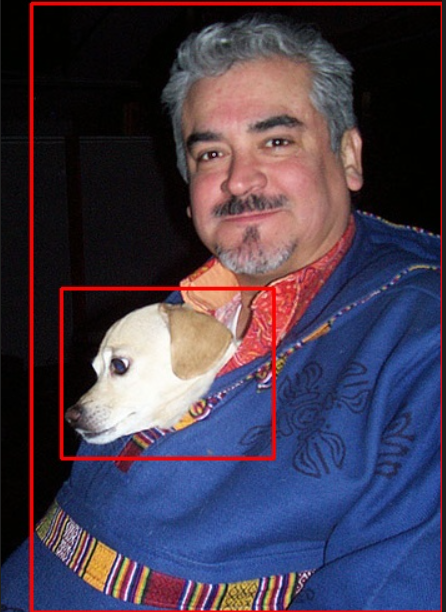
\includegraphics[width=\textwidth]{ssd_result1.png}
        \caption*{\textbf{Image 1:} SSD was able to detect both the person box and dog box despite the overlap.}
    \end{minipage}
    \hfill
    \begin{minipage}[b]{0.45\textwidth}
        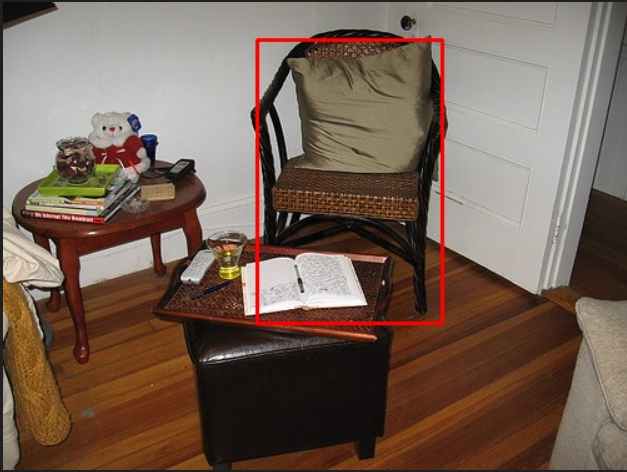
\includegraphics[width=\textwidth]{ssd_result2.png}
        \caption*{\textbf{Image 2:} Also Missed small and distant objects.}
    \end{minipage}
    \caption{Sample predictions using SSD}
\end{figure}

\subsection*{Faster R-CNN Results}

\begin{figure}[H]
    \centering
    \begin{minipage}[b]{0.45\textwidth}
        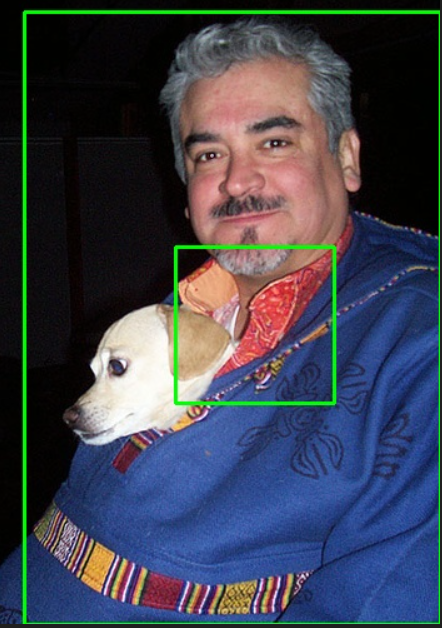
\includegraphics[width=\textwidth]{rcnn_result1.png}
        \caption*{\textbf{Image 1:} detected the person but a false postive missing the dog.}
    \end{minipage}
    \hfill
    \begin{minipage}[b]{0.45\textwidth}
        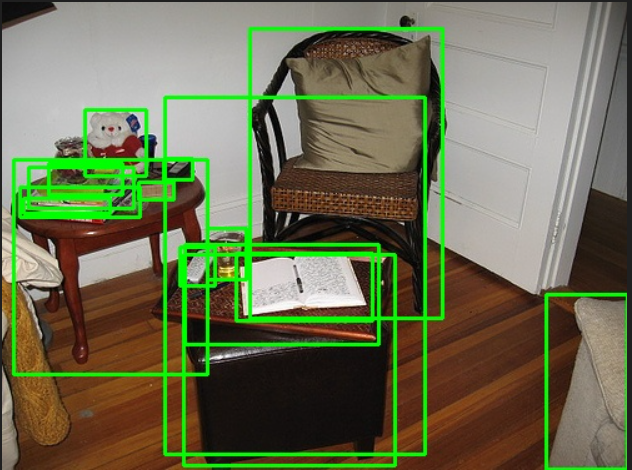
\includegraphics[width=\textwidth]{rcnn_result2.png}
        \caption*{\textbf{Image 2:} Accurately localized small objects even at a distance.}
    \end{minipage}
    \caption{Sample predictions using Faster R-CNN}
\end{figure}

\end{document}

